\section{Theory}\label{sec:the}
During this section we will provide references and briefly describe the main concepts used for performing this research. If you are already familiarised with such topics feel comfortable for skip this section. 

\subsection{SQL Injection}
SQL Injection attacks consists of insertion of specific format of \textit{SQL Queries} via application inputs. The vulnerability happens when these inputs compose SQL queries and are not properly sanitised before executed. A successful SQL Injection attack can perform unauthorised action over the database like: (\textit{i}) read and modify sensitive database data, (\textit{ii}) recover files from filesystem and (\textit{iii}) execute administration operations on the database (such as shutdown the DBMS). 

This type of vulnerability appears on any software which establishes a database connection and has unvalidated data inputs. Code \ref{cod:sqli01} shows us an example of a vulnerable application written using an hypothetic language.

\lstset{frame=single, captionpos=b, numbers=left, stepnumber=1, tabsize=2, basicstyle=\footnotesize\ttfamily,numberstyle=\tiny, numbersep=5pt}
\begin{lstlisting}[caption=SQL Injection vulnerable code example,label=cod:sqli01]
$a = param["id"];
$query = "SELECT name, surname FROM users WHERE id = " + a;
$rows = $dbmc->execute($query);
\end{lstlisting}

The application showed on Code \ref{cod:sqli01} receives an parameter called ``\textit{id}'', concatenate it without any validation with the string stored inside the variable $\$query$ in order to assembly the SQL Query then execute this query through a databased connection object stored inside variable $\$dbmc$. For exploiting such kind of vulnerable application an external user can inject the malicious input showed on Code \ref{cod:sqli02}. 

\begin{lstlisting}[caption=malicious input,label=cod:sqli02]
1 UNION SELECT "x", password FROM users WHERE id = 1 LIMIT 2,1;
\end{lstlisting}

This malicious input induce the application to return the ``\textit{password}'' column content instead the ``\textit{surname}'' one for the user with ``id'' equal to ``1''.

This was a really simple example to illustrate how a SQL Injection attack works the basic concept is the same for all experimentation scenarios that will be presented during Section \ref{sec:exp}. For a deeper understanding about SQL Injection vulnerabilities we strongly recommend the reading of the book ``The Web Application Hacker's Handbook: Finding and Exploiting Security Flaws'' \cite{Stuttard2011, Clarke2012} and some specific papers \cite{Dougherty2011, Puppy1998}.

\subsection{Taint Analysis}
Taint analysis is specific category of Data Flow Analysis. The philosophy behind Taint is that any variable that can be modified by an external user represents a security risk \cite{Schwartz2010,Tang2010,Zhang2011}. This technique was introduced by Perl Programming language developers since $1989$ \cite{Perl1989} for debugging purposes. The first commercial use of Taint Checking was implemented by Netscape for testing its navigator on $1996$.

Taint analysis has basically three main steps:

\begin{itemize}
	\item Taint introduction: determine software input;
	\item Taint Propagation: determine a set of tainted variables due to a specific input;
	\item Taint Enforcement: determine transitions rules to be verified along the taint process. 
\end{itemize}

Taint analysis has two main approaches: (\textit{i}) dynamically and (\textit{ii}) statically. For this research we are specifically interested on the last one. As we do not have execution time information, input sources has to be pointed by some heuristic or an analyst in order to perform the analysis properly.

Code \ref{cod:tai01} show us a simple piece of code for illustrate the static taint analysis process. This example presents three functions: ``\textit{main}'', ``\textit{sanitize}'' and ``\textit{produce\_sql}''. The ``\textit{main}'' procedure is the first one to be executed receiving an input data as parameter through the ``\textit{input\_01}'' variable.

\begin{lstlisting}[caption=Example code for Taint Analysis,label=cod:tai01]
	def produce_sql (param)
		t0 = "select * from users where id = " + sanitize(param)
		return  t0
	end

	def sanitize (num)
		return (int) num;
	end

	def main (input_01)
		id = input_01;
		
		if (id > 1)
			rows = $dbms->execute(produce_sql(id))
		else
			t1 = "Error: id (" + id + ") should be greater than zero"
			puts(t1);
			return -1;
		end
		...
	end
\end{lstlisting}

Analysing the flow of this code we can determine which variables are influenced by the input parameter (taint propagation). Using a forward approach we can mount the graph showed at Figure \ref{fig:taint01} (a). This graph means that the variable ``\textit{t0}'' receives influence from the input parameter ``\textit{input\_01}'' through the bolded path. If we invert the direction of the edges we got the backward analysis from some point inside the code. Figure \ref{fig:taint01} (b) show us a backward taint analysis for the variable ``\textit{produce\_sql:t0}'' where the bolded path indicates that the input variable ``\textit{input\_01}'' is tainted by the variable ``\textit{t0}''.

There are a lot of complexities in build such flow graph over complex and multi-modules code once its reasonable that user data inputs are used for several computations through the code. Other complexity is related to automatic input identification once the code is never executed and we don't have any execution-time information.

\begin{figure}[ht]
\centering
\subfloat[]{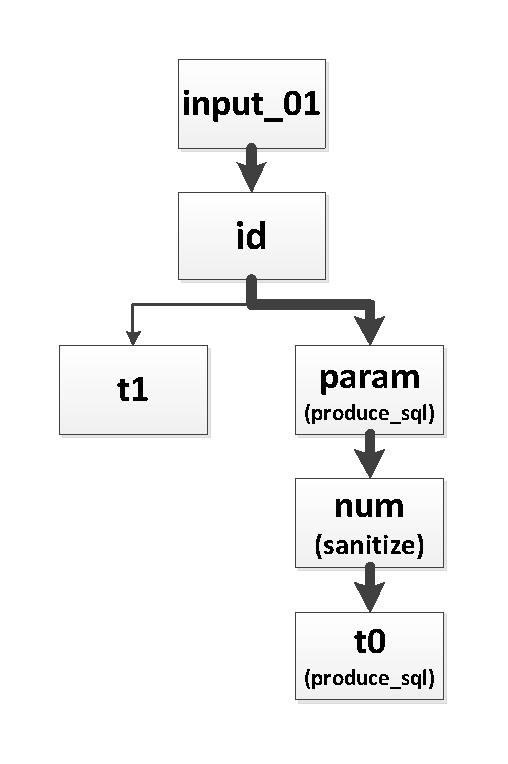
\includegraphics[width=0.45\textwidth]{image/taint_analysis_graph.pdf}}
\subfloat[]{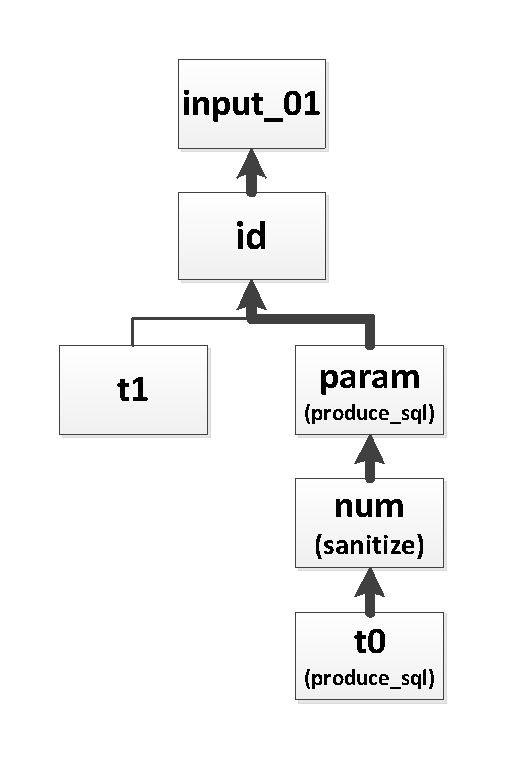
\includegraphics[width=0.45\textwidth]{image/backward_taint_analysis_graph.pdf}}
\caption{Taint analysis graph (a) forward and (b) backward}
\label{fig:taint01}
\end{figure}

This research is interested on backward taint analysis for verify the relationship between variables used inside composed strings used as queries and user input variables. 
